\documentclass[conference]{IEEEtran}
\IEEEoverridecommandlockouts
\usepackage{cite}
\usepackage{amsmath,amssymb,amsfonts}
\usepackage{algorithmic}
\usepackage{graphicx}
\usepackage{textcomp}
\usepackage{xcolor}
\usepackage{booktabs}
\usepackage{url}
\def\BibTeX{{\rm B\kern-.05em{\sc i\kern-.025em b}\kern-.08em
    T\kern-.1667em\lower.7ex\hbox{E}\kern-.125emX}}
\graphicspath{{figures/}}
\renewcommand{\tablename}{Tabel}
\renewcommand{\figurename}{Gambar}
\renewcommand{\IEEEkeywordsname}{Kata kunci}
\renewcommand{\abstractname}{Abstrak}
\renewcommand{\refname}{Daftar Pustaka}
\begin{document}

\title{Reproduksi Iterated Tabu Search untuk Multi-Compartment Truck and Trailer Routing Problem dan Perbandingannya dengan Genetic Algorithm dan Particle Swarm Optimization}

\author{\IEEEauthorblockN{Muhammad Faishal Dienul Haq}
\IEEEauthorblockA{NIM 28426006}
\and
\IEEEauthorblockN{Naufal Izza Fikry}
\IEEEauthorblockA{NIM 28426013}
}

\maketitle

\begin{abstract}
Laporan ini mereproduksi heuristik dua fase Davila-Pena dkk.\ untuk persoalan rute truk dan trailer dengan kendaraan multi-kompartemen, yang berasal dari distribusi pakan sebuah koperasi di Spanyol, lalu membandingkannya dengan Genetic Algorithm dan Particle Swarm Optimization. Heuristik makalah, yaitu Clarke--Wright yang dilanjutkan iterated tabu search, dijalankan dengan kode R asli penulis setelah lima masalah teknis diperbaiki, termasuk pembacaan memori di luar batas pada fungsi penalti. GA dengan dua operator crossover (OX dan PMX) dan PSO berbasis random key memakai satu decoder split yang selalu menghasilkan rute valid. Ketiga algoritma diuji pada delapan instance data nyata dan enam instance benchmark Chao, masing-masing 10 run dengan batas waktu yang sama. Biaya solusi awal sama persis dengan makalah, dan solusi tabu search terbaik berada dalam rentang 1,1 persen dari nilai yang dilaporkan. Tabu search memberikan rata-rata terbaik pada semua instance benchmark. GA berada di urutan kedua dan sesekali menemukan solusi lebih pendek daripada nilai terbaik di makalah, sedangkan PSO tertinggal 21 sampai 41 persen. Pada data nyata, GA paling konsisten dan menemukan optimum di tujuh dari delapan instance. Kami juga menemukan dua ketidaksesuaian antara model matematis dan hasil makalah, yaitu aturan armada dan parkir trailer, yang perlu ditetapkan sebelum metode lain dibandingkan.
\end{abstract}

\begin{IEEEkeywords}
truck and trailer routing problem, kendaraan multi-kompartemen, tabu search, genetic algorithm, particle swarm optimization, reproduksi
\end{IEEEkeywords}

\section{Pendahuluan}

Sebuah koperasi pakan ternak di Galicia, Spanyol, melayani lebih dari 1.500 peternak dengan sekitar 40 pesanan per hari \cite{davila2023}. Sebagian peternakan tidak dapat dimasuki kendaraan besar, sehingga pengiriman memakai truk yang dapat menarik trailer: trailer ditinggal di titik parkir, lalu truk melanjutkan perjalanan sendiri ke pelanggan yang aksesnya sempit. Koperasi ini juga mengirim beberapa jenis pakan yang tidak boleh dicampur, dan satu kompartemen (\textit{hopper}) tidak boleh diisi untuk dua pelanggan karena tidak ada alat takar di atas kendaraan. Davila-Pena dkk.\ \cite{davila2023} memodelkan persoalan ini sebagai \textit{Multi-Compartment Truck and Trailer Routing Problem} (MC-TTRP), yaitu gabungan \textit{truck and trailer routing problem} (TTRP) \cite{chao2002} dengan kendaraan multi-kompartemen \cite{ostermeier2021}.

Model eksak MC-TTRP sulit diselesaikan. Dengan Gurobi, instance 10 pelanggan membutuhkan 31,2 jam, dan instance 11 pelanggan tidak selesai dalam dua minggu \cite{davila2023}. Karena itu penulis mengusulkan heuristik dua fase: algoritma Clarke--Wright (CW) yang dimodifikasi untuk membangun solusi awal, lalu \textit{iterated tabu search} (ITS) untuk memperbaikinya. Di bagian kesimpulan, penulis menyarankan metaheuristik lain, misalnya algoritma evolusioner, dibandingkan dengan solusi mereka sebagai tolok ukur.

Laporan ini menindaklanjuti saran tersebut dengan memodelkan MC-TTRP sebagai persoalan pencarian untuk sebuah \textit{problem solving agent}. Kontribusinya adalah sebagai berikut.
\begin{enumerate}
\item Reproduksi ITS memakai kode sumber asli penulis pada data yang sama, termasuk perbaikan lima masalah yang mencegah kode berjalan atau membuat hasilnya tidak terdefinisi.
\item Implementasi \textit{Genetic Algorithm} (GA) dengan dua operator \textit{crossover} (OX dan PMX) dan \textit{Particle Swarm Optimization} (PSO) berbasis \textit{random key}. Keduanya memakai satu \textit{decoder} yang selalu menghasilkan rute valid.
\item Perbandingan ketiga algoritma dengan anggaran waktu yang sama pada 14 instance, 10 \textit{seed} per algoritma, disertai uji Wilcoxon \textit{rank-sum}, kurva konvergensi, dan analisis sensitivitas parameter.
\item Pemeriksa kelayakan (\textit{feasibility checker}) independen yang menghitung ulang biaya setiap solusi akhir, termasuk solusi dari kode R asli.
\end{enumerate}

Bagian~\ref{sec:pustaka} meninjau pustaka terkait. Bagian~\ref{sec:formulasi} merumuskan persoalan. Bagian~\ref{sec:metode} menjelaskan ketiga algoritma, dan Bagian~\ref{sec:desain} menjelaskan desain eksperimen. Hasil dan pembahasannya ada di Bagian~\ref{sec:hasil} dan~\ref{sec:diskusi}.

\section{Tinjauan Pustaka}\label{sec:pustaka}

\textit{Truck and trailer routing problem} diperkenalkan oleh Chao \cite{chao2002}, yang membedakan pelanggan kendaraan (\textit{vehicle customer}, VC) yang dapat dilayani truk bertrailer dan pelanggan truk (\textit{truck customer}, TC) yang hanya dapat dilayani truk tanpa trailer. Chao menyelesaikannya dengan heuristik konstruksi dan \textit{tabu search}, dan menyusun 21 instance benchmark dari instance VRP Christofides. Instance tersebut menjadi dasar banyak penelitian lanjutan: Scheuerer \cite{scheuerer2006} memakai \textit{tabu search}, Lin dkk.\ \cite{lin2009} memakai \textit{simulated annealing}, Caramia dan Guerriero \cite{caramia2010a} menggabungkan pemrograman matematis dengan \textit{local search}, dan Derigs dkk.\ \cite{derigs2013} memakai \textit{local search} dan \textit{large neighborhood search}.

Pada sisi kendaraan multi-kompartemen, El Fallahi dkk.\ \cite{elfallahi2008} membandingkan algoritma memetika dan \textit{tabu search}, dan mendapati \textit{tabu search} sedikit lebih baik dengan waktu komputasi lebih lama. Silvestrin dan Ritt \cite{silvestrin2017} mengusulkan ITS untuk MC-VRP, yang kemudian menjadi salah satu dasar ITS dalam \cite{davila2023}. Ostermeier dkk.\ \cite{ostermeier2021} menyusun tipologi MC-VRP. Satu-satunya penelitian sebelum \cite{davila2023} yang menggabungkan trailer dan kompartemen adalah Caramia dan Guerriero \cite{caramia2010b} untuk pengumpulan susu.

Untuk GA pada persoalan rute, Prins \cite{prins2004} menunjukkan bahwa kromosom berupa permutasi pelanggan tanpa pemisah rute (\textit{giant tour}) dapat dipecah menjadi rute secara optimal dengan prosedur \textit{split} berbasis lintasan terpendek. Operator \textit{crossover} yang umum untuk permutasi antara lain \textit{order crossover} (OX) \cite{davis1985} dan \textit{partially mapped crossover} (PMX) \cite{goldberg1985}. PSO diperkenalkan oleh Kennedy dan Eberhart \cite{kennedy1995} untuk ruang kontinu, dan bobot inersia ditambahkan oleh Shi dan Eberhart \cite{shi1998}. Untuk persoalan urutan, representasi \textit{random key} \cite{bean1994} memetakan vektor kontinu menjadi permutasi dengan mengurutkan nilainya, sehingga persamaan PSO standar dapat dipakai tanpa diubah.

\section{Formulasi Persoalan}\label{sec:formulasi}

\subsection{Deskripsi MC-TTRP}

Diberikan graf lengkap $G=(N,E)$ dengan $N=\{0,1,\dots,n\}$, simpul 0 adalah depot, dan $c_{ij}$ adalah jarak antara simpul $i$ dan $j$. Himpunan pelanggan terbagi menjadi VC ($N_1$) dan TC ($N_2$). Pelanggan $i$ meminta $d_{if}$ unit produk $f\in F$. Tersedia $m_T$ truk dan $m_L\le m_T$ trailer. Setiap truk memiliki $|H^T|$ \textit{hopper} berkapasitas $Q_T^H$, dan setiap trailer memiliki $|H^L|$ \textit{hopper} berkapasitas $Q_L^H$. Satu \textit{hopper} hanya boleh berisi satu produk milik satu pelanggan, tetapi permintaan satu pelanggan boleh dipecah ke beberapa \textit{hopper}.

Solusi terdiri dari rute dengan tiga tipe \cite{chao2002,davila2023}:
\begin{itemize}
\item \textit{pure truck route} (PTR): truk tanpa trailer, boleh melayani VC dan TC;
\item \textit{pure vehicle route} (PVR): truk dan trailer sepanjang rute, hanya melayani VC;
\item \textit{mixed vehicle route} (MVR): \textit{main tour} truk bertrailer yang melayani VC. Di sebuah VC pada \textit{main tour}, trailer diparkir dan truk menjalani satu atau lebih \textit{sub-tour} sendirian untuk melayani VC atau TC, lalu kembali mengambil trailer.
\end{itemize}

Tujuannya adalah meminimalkan total jarak tempuh semua rute, yaitu persamaan (1) pada \cite{davila2023}:
\begin{equation}
\min \; f(S) = \sum_{r\in S}\Bigl(\sum_{(i,j)\in \text{main}(r)} c_{ij} + \sum_{t\in \text{sub}(r)}\;\sum_{(i,j)\in t} c_{ij}\Bigr).\label{eq:obj}
\end{equation}
Batasannya: setiap pelanggan dilayani tepat satu kali, TC tidak berada di \textit{main tour}, muatan \textit{sub-tour} hanya boleh diangkut di \textit{hopper} truk, setiap kombinasi pelanggan dan produk harus masuk \textit{hopper} sesuai aturan di atas, dan jumlah kendaraan tidak melebihi armada.

\subsection{Aturan armada dan parkir trailer}\label{sec:armada}

Model MILP pada \cite{davila2023} melarang truk yang dapat menarik trailer menjalankan PTR (batasan (10)), sehingga jumlah PTR paling banyak $m_T-m_L$. Namun, hasil yang dilaporkan pada Tabel 4 makalah tersebut melanggar batasan ini. Contohnya, instance 2 memakai 8 truk, 4 trailer, dan 4 PTR, padahal $m_T-m_L=8-5=3$. Kode R asli juga menghasilkan solusi seperti itu. Kami memakai aturan yang sesuai dengan heuristik dan hasil penulis, dan aturan yang sama berlaku untuk semua algoritma:
\begin{equation}
n_{\text{PVR}}+n_{\text{MVR}}\le m_L, \qquad n_{\text{PVR}}+n_{\text{MVR}}+n_{\text{PTR}}\le m_T.\label{eq:fleet}
\end{equation}
Teks makalah menyebut depot sebagai calon tempat parkir trailer, tetapi batasan (10) juga melarang rute berakar di depot untuk truk bertrailer. Nilai optimum Gurobi dihitung dengan model tersebut, dan kode ITS asli tidak pernah memarkir trailer di depot (0 dari 290 MVR pada eksperimen kami). Karena itu \textit{sub-tour} hanya boleh berakar di VC pada \textit{main tour}. Pada percobaan awal yang masih mengizinkan parkir di depot, GA menghasilkan biaya di bawah optimum Gurobi pada lima instance P (misalnya 199 km pada P6, sedangkan optimumnya 222 km), sehingga aturan ini jelas mengubah persoalan. Batas waktu kerja pengemudi pada model tidak diimplementasikan dalam kode asli, sehingga juga tidak dipakai di sini.

\subsection{Rumusan sebagai persoalan pencarian}

Untuk ketiga algoritma, komponen persoalan pencarian adalah sebagai berikut.
\begin{itemize}
\item \textbf{State}: solusi lengkap, yaitu himpunan rute beserta tipenya dan alokasi muatan ke \textit{hopper}. Pada GA dan PSO, \textit{state} dikodekan sebagai permutasi pelanggan $\pi$ yang diterjemahkan oleh \textit{decoder} (Bagian~\ref{sec:decoder}).
\item \textbf{Fungsi biaya}: total jarak \eqref{eq:obj}. Selama pencarian, pelanggaran batasan diberi penalti (Bagian~\ref{sec:metode}). Hasil akhir selalu dilaporkan sebagai jarak murni dari solusi yang valid.
\item \textbf{Operator}: pada ITS berupa gerakan \textit{local search} (\textit{relocate}, \textit{exchange}, 2-opt, 2-opt*, dan gerakan khusus \textit{sub-tour}). Pada GA berupa seleksi, \textit{crossover}, dan mutasi pada permutasi. Pada PSO berupa pembaruan kecepatan dan posisi.
\item \textbf{Goal}: tidak ada \textit{goal state} eksplisit. Pencarian berhenti saat anggaran habis, lalu mengembalikan solusi valid terbaik.
\end{itemize}

Kualitas solusi diukur dengan \textit{gap} terhadap nilai acuan $z^{\text{ref}}$:
\begin{equation}
\text{gap} = \frac{z - z^{\text{ref}}}{z^{\text{ref}}}\times 100\%.\label{eq:gap}
\end{equation}

\section{Metode}\label{sec:metode}

\subsection{Baseline: Clarke--Wright dan Iterated Tabu Search}

Baseline adalah heuristik dari \cite{davila2023}, dijalankan dengan kode R asli penulis\footnote{\url{https://github.com/LauraDavilaPena/ITS_MC-TTRP}, versi 0.1, lisensi GPLv3.}. Fase pertama adalah algoritma CW dengan dua matriks penghematan: penghematan biasa $s_{ij}=c_{i0}+c_{0j}-c_{ij}$ dan penghematan untuk mengubah rute TC menjadi \textit{sub-tour} yang berakar di sebuah VC. Solusi CW kemudian diperbaiki dengan 2-opt, 3-opt, 4-opt*, dan gerakan \textit{local search}.

Fase kedua adalah ITS. Pada setiap iterasi, solusi diperturbasi dengan mengeluarkan dan menyisipkan kembali $\phi$ pelanggan acak, dengan $\phi$ sebesar 1--10\% dari $n$. Setelah itu dijalankan \textit{tabu search} yang memilih gerakan terbaik di seluruh \textit{neighborhood}, meskipun gerakan itu memperburuk solusi atau membuatnya tidak layak. Biaya rute selama \textit{tabu search} adalah
\begin{equation}
F(r) = d(r) + \alpha\, C(r),\label{eq:tabu}
\end{equation}
dengan $d(r)$ jarak dan $C(r)$ kelebihan muatan. Nilai $\alpha$ dikali $(1+\gamma)$ bila solusi tidak layak dan dibagi $(1+\gamma)$ bila layak, dengan $\gamma\sim U[0,1]$. Lama keanggotaan dalam daftar tabu diambil dari $U[1,\sqrt{n\cdot nr}]$, dengan $nr$ jumlah rute. Dengan peluang $(\text{iter}/\text{max\_iter})^2$, pencarian kembali ke solusi layak terbaik. Seperti pada makalah, ITS dijalankan 100 iterasi.

Lima masalah pada kode asli kami perbaiki agar kode dapat dijalankan di macOS dengan R 4.6.1:
\begin{enumerate}
\item Kode memuat \texttt{itsmcttrp.dll}, berkas khusus Windows. Kami menyusun ulang \texttt{movlist.cpp} menjadi pustaka untuk sistem operasi yang dipakai.
\item Operator \texttt{\&\&} dan \texttt{||} pada vektor menghasilkan galat sejak R 4.3, sedangkan kode ditulis untuk R 4.0.2 yang diam-diam memakai elemen pertama. Penyebabnya, kapasitas kendaraan disimpan sebagai vektor berisi nilai yang sama untuk setiap trailer. Kami mengembalikan perilaku R 4.0 untuk kedua operator tersebut.
\item Fungsi penalti C++ \texttt{calc\_penalty\_route\_MCTTRP} membaca kolom permintaan $j{+}1$ untuk $j=0,\dots,n_F{-}1$. Akibatnya produk pertama terlewat dan memori di luar matriks ikut terbaca. Kesalahan ini memengaruhi $C(r)$ pada \eqref{eq:tabu} dan kami perbaiki menjadi kolom $j$.
\item Skrip reproduksi tidak memuat kode solver.
\item Skrip untuk data nyata mencetak hasil dari variabel yang tidak didefinisikan.
\end{enumerate}
Kami juga menambahkan pencatatan biaya terbaik per iterasi untuk kurva konvergensi. Perbaikan nomor 3 berarti versi yang kami jalankan tidak identik dengan biner yang dipakai penulis.

\subsection{Decoder giant tour}\label{sec:decoder}

GA dan PSO bekerja pada permutasi pelanggan $\pi=(\pi_1,\dots,\pi_n)$. \textit{Decoder} memotong $\pi$ menjadi segmen berurutan, dengan satu segmen menjadi satu rute, mengikuti gagasan \textit{split} \cite{prins2004}. Segmen $\pi_{i+1..j}$ dapat menjadi:
\begin{itemize}
\item PTR, bila seluruh muatannya muat di \textit{hopper} truk;
\item PVR, bila segmen tidak berisi TC dan muatannya muat di truk dan trailer;
\item MVR, bila segmen berisi VC dan TC. VC membentuk \textit{main tour} dan TC membentuk satu \textit{sub-tour} yang berakar di VC segmen dengan biaya sisip terkecil.
\end{itemize}
Kelayakan muatan diperiksa secara eksak dengan pemrograman dinamis atas jumlah \textit{hopper} trailer yang terpakai: setiap permintaan $d_{if}$ boleh dibagi ke $x$ \textit{hopper} trailer dan $y=\lceil (d_{if}-xQ_L^H)/Q_T^H\rceil$ \textit{hopper} truk.

Misalkan $V(j,a,b)$ adalah biaya minimum untuk melayani $\pi_1,\dots,\pi_j$ dengan $a$ kendaraan bertrailer dan $b$ PTR. Rekurensinya
\begin{equation}
V(j,a,b)=\min_{i<j}\Bigl\{V(i,a{-}1,b)+c^{\text{K}}_{ij},\; V(i,a,b{-}1)+c^{\text{T}}_{ij}\Bigr\},\label{eq:split}
\end{equation}
dengan $c^{\text{K}}_{ij}$ biaya segmen sebagai PVR atau MVR dan $c^{\text{T}}_{ij}$ biaya sebagai PTR. Nilainya $\infty$ bila segmen tidak layak untuk tipe tersebut. Bila tidak ada pemotongan yang memenuhi \eqref{eq:fleet}, \textit{decoder} mengizinkan hingga tiga kendaraan tambahan dengan penalti
\begin{equation}
P = 2n\max_{i,j}c_{ij} + 1\label{eq:pen}
\end{equation}
per kendaraan berlebih. Nilai $P$ lebih besar dari biaya solusi layak mana pun, sehingga solusi layak selalu lebih baik daripada solusi tak layak, sementara solusi tak layak tetap dapat diperingkat. Solusi layak terbaik dicatat terpisah. Satu evaluasi membutuhkan sekitar 0,1 ms untuk 50--75 pelanggan.

Satu \textit{sub-tour} per MVR adalah penyederhanaan dibanding model asli yang mengizinkan beberapa \textit{sub-tour}. Penyederhanaan ini membuat ruang solusi GA dan PSO lebih kecil daripada ruang solusi ITS.

\subsection{Genetic Algorithm}

Kromosom adalah permutasi pelanggan, dan \textit{fitness} adalah biaya hasil \textit{decoder}. Populasi awal dibangkitkan acak. Orang tua dipilih dengan turnamen berukuran $k=3$, yang memberi tekanan seleksi sedang tanpa perlu menskalakan \textit{fitness}. Dua variasi \textit{crossover} dibandingkan, sesuai ketentuan tugas:
\begin{itemize}
\item \textbf{OX} \cite{davis1985}: segmen $[a,b]$ dari orang tua pertama disalin ke posisi yang sama, lalu sisa posisi diisi dengan urutan relatif gen orang tua kedua mulai dari $b+1$. OX mempertahankan urutan relatif, yang relevan karena \textit{decoder} memotong permutasi menjadi segmen berurutan.
\item \textbf{PMX} \cite{goldberg1985}: segmen yang sama disalin, lalu gen orang tua kedua di jendela tersebut dipetakan lewat pasangan $p_1[i]\leftrightarrow p_2[i]$. PMX lebih mempertahankan posisi absolut gen.
\end{itemize}
Mutasi berupa inversi segmen acak. Inversi hanya mengubah dua sisi pada urutan kunjungan, sehingga cocok untuk objektif berbasis jarak. Dua individu terbaik disalin langsung ke generasi berikutnya (elitisme).

Parameter yang dipakai: ukuran populasi 100, peluang \textit{crossover} 0,9, peluang mutasi 0,2, elitisme 2. Ukuran populasi 100 memberi sekitar 100 generasi per 10 detik pada instance 50 pelanggan. Peluang \textit{crossover} 0,9 adalah nilai yang lazim. Peluang mutasi adalah parameter yang paling kami ragukan, sehingga dianalisis sensitivitasnya (Bagian~\ref{sec:sens}).

\subsection{Particle Swarm Optimization}

PSO dipilih sebagai algoritma \textit{swarm intelligence} karena persamaannya dapat dipakai tanpa diubah dengan representasi \textit{random key}. ACO juga cocok untuk persoalan rute, tetapi membutuhkan konstruksi solusi yang memahami tipe rute, trailer, dan kompartemen, sehingga sulit memakai \textit{decoder} yang sama. Dengan \textit{decoder} yang sama, perbedaan hasil GA dan PSO berasal dari strategi pencarian, bukan dari cara membangun rute.

Setiap partikel memiliki posisi $\mathbf{x}\in[0,1]^n$, dan permutasinya adalah $\pi=\operatorname{argsort}(\mathbf{x})+1$ \cite{bean1994}. Pembaruan mengikuti PSO \textit{global best} dengan bobot inersia \cite{kennedy1995,shi1998}:
\begin{align}
\mathbf{v} &\leftarrow w\mathbf{v} + c_1\mathbf{r}_1\odot(\mathbf{p}-\mathbf{x}) + c_2\mathbf{r}_2\odot(\mathbf{g}-\mathbf{x}),\label{eq:vel}\\
\mathbf{x} &\leftarrow \operatorname{clip}\bigl(\mathbf{x}+\operatorname{clip}(\mathbf{v},-v_{\max},v_{\max}),\,0,\,1\bigr),\label{eq:pos}
\end{align}
dengan $\mathbf{p}$ posisi terbaik partikel, $\mathbf{g}$ posisi terbaik kawanan, dan $\mathbf{r}_1,\mathbf{r}_2\sim U(0,1)^n$. Bobot inersia turun linear terhadap fraksi anggaran yang sudah terpakai, $\tau\in[0,1]$:
\begin{equation}
w(\tau)=w_{\text{start}}+(w_{\text{end}}-w_{\text{start}})\,\tau.\label{eq:inertia}
\end{equation}
Parameter yang dipakai: 50 partikel, $w_{\text{start}}=0{,}9$, $w_{\text{end}}=0{,}4$, $c_1=c_2=2$, dan $v_{\max}=0{,}2$. Nilai $c_1=c_2=2$ mengikuti \cite{kennedy1995}. Batas $v_{\max}$ sebesar 20\% rentang kunci mencegah kunci menumpuk di batas 0 atau 1, karena kunci yang menumpuk membuat permutasi berhenti berubah. Nilai $w_{\text{end}}$ dianalisis sensitivitasnya.

\section{Desain Eksperimen}\label{sec:desain}

\subsection{Data}

Semua algoritma memakai berkas instance yang sama dari repositori penulis. Kesamaan berkas diperiksa dengan \textit{hash} SHA-256 dalam pengujian otomatis.
\begin{itemize}
\item \textbf{P1--P8}: data nyata koperasi dengan 8--10 pelanggan, 4 jenis pakan, 2 truk (13 \textit{hopper} @1.500 kg), dan 1 trailer (15 \textit{hopper} @2.000 kg). Jaraknya dalam km. Nilai acuan adalah solusi eksak Gurobi pada Tabel 5 \cite{davila2023}.
\item \textbf{C01--C06}: instance Chao \cite{chao2002} yang diberi kompartemen oleh penulis, dengan 50 pelanggan (C01--C03) dan 75 pelanggan (C04--C06). Proporsi TC adalah 25\%, 50\%, dan 75\% berturut-turut. Truk memiliki 20 \textit{hopper} berkapasitas 5, dan trailer memiliki 10 \textit{hopper} berkapasitas 10. Jaraknya Euklides. Belum ada solusi optimal untuk instance ini, sehingga nilai acuannya adalah hasil ITS terbaik dari 10 run pada Tabel 4 \cite{davila2023}.
\end{itemize}
Jumlah truk dan trailer mengikuti skrip reproduksi penulis: (2,1) untuk P1--P8, (8,5) untuk C01--C03, (13,8) untuk C04, dan (14,8) untuk C05--C06. Instance Chao 07--21 tidak dipakai karena satu run ITS pada instance tersebut membutuhkan 17--93 menit \cite{davila2023}, sehingga tidak dapat diselesaikan sebelum tenggat tugas.

\subsection{Anggaran dan pengaturan}

Setiap algoritma dijalankan 10 kali per instance dengan \textit{seed} 1--10. ITS dijalankan 100 iterasi, sesuai makalah. GA dan PSO diberi batas waktu \textit{wall-clock} yang sama dengan rata-rata waktu ITS pada instance yang sama. Waktu dipilih sebagai anggaran, bukan jumlah evaluasi, karena satu evaluasi gerakan pada ITS dan satu evaluasi permutasi utuh pada GA/PSO berbeda besarnya. Semua run dijalankan di satu komputer Apple M5 (10 inti) dengan 8 proses paralel. GA dan PSO ditulis dalam Python 3.14 dengan numba, sedangkan ITS ditulis dalam R dan C++.

Untuk setiap instance dan algoritma, kami melaporkan biaya terbaik, rata-rata, simpangan baku, dan terburuk, serta \textit{gap} \eqref{eq:gap}. Setiap solusi akhir diperiksa ulang oleh pemeriksa kelayakan independen yang menguji cakupan pelanggan, tipe pelanggan, armada \eqref{eq:fleet}, dan muatan \textit{hopper} secara eksak, lalu biayanya dihitung ulang. Pemeriksa ini lolos uji pada solusi optimal yang dicetak di Bagian 5.1 makalah, yang bernilai 207 km. Perbedaan antaralgoritma diuji dengan Wilcoxon \textit{rank-sum} dua sisi \cite{wilcoxon1945} pada $\alpha=0{,}05$. Analisis sensitivitas dilakukan pada C01 dengan 5 \textit{seed} untuk peluang mutasi GA-OX $\in\{0{,}05;0{,}1;0{,}2;0{,}4\}$ dan $w_{\text{end}}$ PSO $\in\{0{,}2;0{,}4;0{,}6;0{,}8\}$.

\section{Hasil}\label{sec:hasil}

\subsection{Reproduksi ITS}

\begin{table*}[t]
\caption{Reproduksi heuristik dua fase: nilai di makalah \cite{davila2023} dibandingkan dengan 10 run kode asli (selisih = terbaik kami terhadap ITS makalah)}
\label{tab:repro}
\centering\footnotesize
\begin{tabular}{lrrrrrrrr}
\toprule
& \multicolumn{2}{c}{CW} & \multicolumn{3}{c}{ITS} & & \multicolumn{2}{c}{Waktu per run (s)}\\
\cmidrule(lr){2-3}\cmidrule(lr){4-6}\cmidrule(lr){8-9}
Instance & Makalah & Kami & Makalah & Terbaik kami & Rata-rata kami & Selisih (\%) & Makalah & Kami\\
\midrule
P1 & -- & 189,00 & 189,00 & 189,00 & 189,00 & 0,00 & 5,0 & 7,5 \\
P2 & -- & 143,00 & 142,00 & 140,00 & 141,40 & -1,41 & 3,9 & 7,3 \\
P3 & -- & 106,00 & 106,00 & 106,00 & 106,00 & 0,00 & 3,9 & 7,0 \\
P4 & -- & 256,00 & 256,00 & 256,00 & 256,00 & 0,00 & 5,6 & 8,4 \\
P5 & -- & 110,00 & 109,00 & 109,00 & 109,00 & 0,00 & 4,7 & 8,0 \\
P6 & -- & 226,00 & 223,00 & 222,00 & 224,10 & -0,45 & 6,5 & 9,4 \\
P7 & -- & 238,00 & 238,00 & 237,00 & 237,00 & -0,42 & 8,0 & 9,2 \\
P8 & -- & 213,00 & 213,00 & 207,00 & 212,30 & -2,82 & 6,1 & 7,8 \\
C01 & 662,93 & 662,94 & 640,66 & 633,61 & 640,08 & -1,10 & 334,8 & 307,9 \\
C02 & 832,60 & 832,60 & 708,08 & 711,21 & 723,55 & 0,44 & 316,8 & 263,6 \\
C03 & 885,79 & 885,79 & 764,81 & 761,10 & 777,35 & -0,48 & 345,6 & 277,8 \\
C04 & 1013,57 & 1013,57 & 908,53 & 904,39 & 934,80 & -0,46 & 633,0 & 629,9 \\
C05 & 1168,01 & 1168,01 & 1012,83 & 1012,91 & 1029,39 & 0,01 & 535,8 & 541,7 \\
C06 & 1264,09 & 1264,09 & 1101,90 & 1104,10 & 1143,67 & 0,20 & 847,8 & 585,9 \\

\bottomrule
\end{tabular}
\end{table*}

Tabel~\ref{tab:repro} membandingkan hasil makalah dengan 10 run kode asli. Biaya solusi CW kami sama dengan makalah pada keenam instance Chao (selisih hanya pada digit pembulatan, misalnya 662,94 dan 662,93 pada C01). Karena CW deterministik, kesamaan ini menunjukkan bahwa data dan kode yang kami jalankan sama dengan yang dipakai penulis. Solusi ITS terbaik kami berada antara 1,10\% lebih baik dan 0,44\% lebih buruk daripada nilai makalah. Waktu per run juga sebanding: 264--630 detik di komputer kami, sedangkan makalah melaporkan 317--848 detik.

Pada data nyata P1--P8, ITS terbaik kami mencapai optimum Gurobi di kedelapan instance. Pada P2, P6, P7, dan P8, nilai ini lebih baik daripada hasil heuristik di Tabel 5 makalah (142, 223, 238, dan 213 km). Makalah tidak menyebut berapa run yang dipakai untuk Tabel 5. Rata-rata 10 run kami pada P8 adalah 212,3 km, dekat dengan 213 km di makalah. Kemungkinan besar selisih ini muncul karena kami mengambil hasil terbaik dari 10 run. Perbaikan fungsi penalti C++ juga dapat berpengaruh, tetapi pengaruhnya tidak kami ukur secara terpisah. Secara keseluruhan, hasil makalah dapat direproduksi.

\subsection{Perbandingan ITS, GA, dan PSO}

\begin{table*}[t]
\caption{Hasil 10 run per algoritma. Gap dihitung dengan \eqref{eq:gap} terhadap nilai acuan (optimum Gurobi untuk P1--P8, ITS terbaik makalah untuk C01--C06). Rata-rata terbaik per instance dicetak tebal.}
\label{tab:summary}
\centering\scriptsize
\begin{tabular}{llrrrrrrrr}
\toprule
Instance & Acuan & Algoritma & Terbaik & Rata-rata & Std & Terburuk & Gap terbaik (\%) & Gap rata-rata (\%) & Waktu (s)\\
\midrule
P1 & 189,00 & ITS & 189,00 & \textbf{189,00} & 0,00 & 189,00 & 0,00 & 0,00 & 7,5 \\
 &  & GA-OX & 189,00 & \textbf{189,00} & 0,00 & 189,00 & 0,00 & 0,00 & 7,5 \\
 &  & GA-PMX & 189,00 & \textbf{189,00} & 0,00 & 189,00 & 0,00 & 0,00 & 7,5 \\
 &  & PSO & 189,00 & \textbf{189,00} & 0,00 & 189,00 & 0,00 & 0,00 & 7,5 \\
\midrule
P2 & 140,00 & ITS & 140,00 & 141,40 & 0,97 & 142,00 & 0,00 & 1,00 & 7,3 \\
 &  & GA-OX & 140,00 & \textbf{140,00} & 0,00 & 140,00 & 0,00 & 0,00 & 7,3 \\
 &  & GA-PMX & 140,00 & \textbf{140,00} & 0,00 & 140,00 & 0,00 & 0,00 & 7,3 \\
 &  & PSO & 140,00 & \textbf{140,00} & 0,00 & 140,00 & 0,00 & 0,00 & 7,3 \\
\midrule
P3 & 106,00 & ITS & 106,00 & \textbf{106,00} & 0,00 & 106,00 & 0,00 & 0,00 & 7,0 \\
 &  & GA-OX & 106,00 & \textbf{106,00} & 0,00 & 106,00 & 0,00 & 0,00 & 7,0 \\
 &  & GA-PMX & 106,00 & \textbf{106,00} & 0,00 & 106,00 & 0,00 & 0,00 & 7,0 \\
 &  & PSO & 106,00 & \textbf{106,00} & 0,00 & 106,00 & 0,00 & 0,00 & 7,0 \\
\midrule
P4 & 256,00 & ITS & 256,00 & \textbf{256,00} & 0,00 & 256,00 & 0,00 & 0,00 & 8,4 \\
 &  & GA-OX & 256,00 & \textbf{256,00} & 0,00 & 256,00 & 0,00 & 0,00 & 8,4 \\
 &  & GA-PMX & 256,00 & \textbf{256,00} & 0,00 & 256,00 & 0,00 & 0,00 & 8,4 \\
 &  & PSO & 256,00 & 256,20 & 0,63 & 258,00 & 0,00 & 0,08 & 8,4 \\
\midrule
P5 & 109,00 & ITS & 109,00 & \textbf{109,00} & 0,00 & 109,00 & 0,00 & 0,00 & 8,0 \\
 &  & GA-OX & 109,00 & \textbf{109,00} & 0,00 & 109,00 & 0,00 & 0,00 & 8,0 \\
 &  & GA-PMX & 109,00 & \textbf{109,00} & 0,00 & 109,00 & 0,00 & 0,00 & 8,0 \\
 &  & PSO & 109,00 & 109,40 & 0,84 & 111,00 & 0,00 & 0,37 & 8,0 \\
\midrule
P6 & 222,00 & ITS & 222,00 & \textbf{224,10} & 1,45 & 225,00 & 0,00 & 0,95 & 9,4 \\
 &  & GA-OX & 225,00 & 225,00 & 0,00 & 225,00 & 1,35 & 1,35 & 9,4 \\
 &  & GA-PMX & 225,00 & 225,00 & 0,00 & 225,00 & 1,35 & 1,35 & 9,4 \\
 &  & PSO & 225,00 & 225,50 & 1,58 & 230,00 & 1,35 & 1,58 & 9,4 \\
\midrule
P7 & 237,00 & ITS & 237,00 & \textbf{237,00} & 0,00 & 237,00 & 0,00 & 0,00 & 9,2 \\
 &  & GA-OX & 237,00 & \textbf{237,00} & 0,00 & 237,00 & 0,00 & 0,00 & 9,2 \\
 &  & GA-PMX & 237,00 & \textbf{237,00} & 0,00 & 237,00 & 0,00 & 0,00 & 9,2 \\
 &  & PSO & 237,00 & 237,10 & 0,32 & 238,00 & 0,00 & 0,04 & 9,2 \\
\midrule
P8 & 207,00 & ITS & 207,00 & 212,30 & 1,89 & 213,00 & 0,00 & 2,56 & 7,8 \\
 &  & GA-OX & 207,00 & \textbf{207,00} & 0,00 & 207,00 & 0,00 & 0,00 & 7,8 \\
 &  & GA-PMX & 207,00 & \textbf{207,00} & 0,00 & 207,00 & 0,00 & 0,00 & 7,8 \\
 &  & PSO & 207,00 & 207,60 & 1,90 & 213,00 & 0,00 & 0,29 & 7,8 \\
\midrule
C01 & 640,66 & ITS & 633,61 & \textbf{640,08} & 6,29 & 652,55 & -1,10 & -0,09 & 307,9 \\
 &  & GA-OX & 628,86 & 655,27 & 27,72 & 709,89 & -1,84 & 2,28 & 307,9 \\
 &  & GA-PMX & 652,34 & 675,34 & 16,46 & 702,41 & 1,82 & 5,41 & 307,9 \\
 &  & PSO & 745,40 & 808,76 & 28,99 & 845,46 & 16,35 & 26,24 & 307,9 \\
\midrule
C02 & 708,08 & ITS & 711,21 & \textbf{723,55} & 8,26 & 736,85 & 0,44 & 2,18 & 263,6 \\
 &  & GA-OX & 718,06 & 745,56 & 16,57 & 761,21 & 1,41 & 5,29 & 263,6 \\
 &  & GA-PMX & 714,11 & 753,68 & 22,97 & 782,57 & 0,85 & 6,44 & 263,6 \\
 &  & PSO & 784,57 & 879,00 & 63,14 & 953,35 & 10,80 & 24,14 & 263,6 \\
\midrule
C03 & 764,81 & ITS & 761,10 & \textbf{777,35} & 14,21 & 810,20 & -0,48 & 1,64 & 277,8 \\
 &  & GA-OX & 749,23 & 787,63 & 27,16 & 834,19 & -2,04 & 2,98 & 277,8 \\
 &  & GA-PMX & 759,32 & 808,55 & 35,62 & 888,85 & -0,72 & 5,72 & 277,8 \\
 &  & PSO & 860,59 & 925,44 & 55,45 & 1014,31 & 12,52 & 21,00 & 277,8 \\
\midrule
C04 & 908,53 & ITS & 904,39 & \textbf{934,80} & 28,23 & 990,55 & -0,46 & 2,89 & 629,9 \\
 &  & GA-OX & 911,46 & 961,26 & 30,20 & 1005,77 & 0,32 & 5,80 & 629,9 \\
 &  & GA-PMX & 914,67 & 976,84 & 43,26 & 1075,41 & 0,68 & 7,52 & 629,9 \\
 &  & PSO & 1210,97 & 1277,36 & 42,68 & 1347,94 & 33,29 & 40,60 & 629,9 \\
\midrule
C05 & 1012,83 & ITS & 1012,91 & \textbf{1029,39} & 10,36 & 1046,69 & 0,01 & 1,63 & 541,7 \\
 &  & GA-OX & 1031,38 & 1083,65 & 40,15 & 1145,32 & 1,83 & 6,99 & 541,8 \\
 &  & GA-PMX & 1027,48 & 1078,55 & 43,90 & 1146,63 & 1,45 & 6,49 & 541,8 \\
 &  & PSO & 1217,55 & 1326,97 & 64,59 & 1433,72 & 20,21 & 31,02 & 541,8 \\
\midrule
C06 & 1101,90 & ITS & 1104,10 & \textbf{1143,67} & 18,70 & 1173,84 & 0,20 & 3,79 & 585,9 \\
 &  & GA-OX & 1155,94 & 1208,44 & 49,71 & 1299,82 & 4,90 & 9,67 & 585,9 \\
 &  & GA-PMX & 1154,91 & 1194,90 & 33,81 & 1250,44 & 4,81 & 8,44 & 585,9 \\
 &  & PSO & 1444,51 & 1507,57 & 44,09 & 1593,19 & 31,09 & 36,82 & 585,9 \\

\bottomrule
\end{tabular}
\end{table*}

\begin{figure*}[t]
\centering
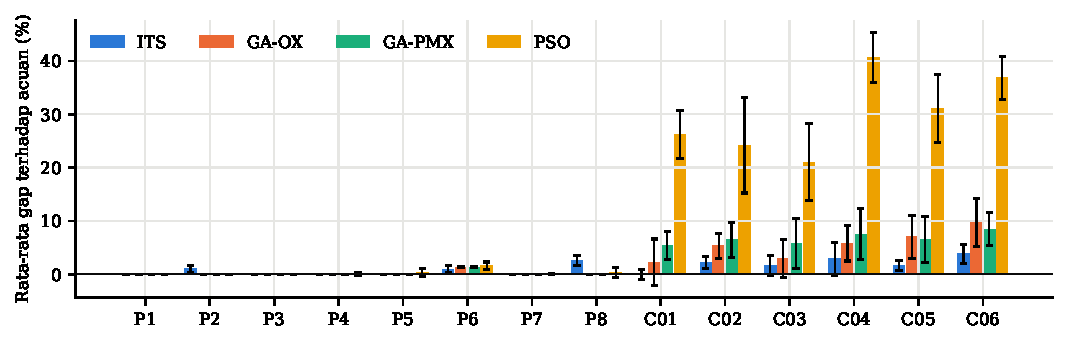
\includegraphics{gap_by_instance.pdf}
\caption{Rata-rata gap setiap algoritma per instance (garis kecil di ujung batang menunjukkan simpangan baku). Makin rendah batang, makin dekat solusinya ke nilai acuan.}
\label{fig:gap}
\end{figure*}

Tabel~\ref{tab:summary} memuat statistik lengkap, dan Gambar~\ref{fig:gap} meringkasnya sebagai diagram batang. Setiap kelompok batang adalah satu instance, dan setiap warna adalah satu algoritma. Tinggi batang adalah rata-rata gap terhadap nilai acuan, jadi batang yang rendah berarti rute rata-ratanya pendek. Batang setinggi nol berarti algoritma selalu menemukan solusi senilai acuan.

Pada data nyata P1--P8, keempat algoritma hampir tidak berbeda. GA-OX dan GA-PMX menemukan optimum di setiap run pada tujuh instance, dengan simpangan baku nol. ITS sedikit kurang konsisten: rata-ratanya 1,0\% di atas optimum pada P2 dan 2,6\% pada P8, karena beberapa run berhenti di solusi 142 km dan 213 km. Satu-satunya instance yang tidak dapat diselesaikan GA dan PSO adalah P6. Ketiganya berhenti di 225 km, sedangkan optimumnya 222 km. Solusi optimal P6 dari ITS memuat VC di dalam \textit{sub-tour} (rute 0-5-4-2-8-7-3-2-1-0, dengan pelanggan 3 dilayani truk dari tempat parkir di pelanggan 2). \textit{Decoder} kami selalu menaruh VC di \textit{main tour}, sehingga solusi ini tidak dapat direpresentasikan.

Pada instance Chao, perbedaannya jelas. ITS memiliki rata-rata terbaik di keenam instance, dengan gap rata-rata antara $-0{,}1\%$ dan 3,8\%. GA berada di urutan berikutnya, dengan gap rata-rata 2,3--9,7\% untuk GA-OX dan 5,4--8,4\% untuk GA-PMX. PSO tertinggal jauh, dengan gap rata-rata 21--41\%. Batang kuning yang menjulang di Gambar~\ref{fig:gap} memperlihatkan selisih ini. Ada satu hal menarik: solusi terbaik GA-OX pada C01 (628,86) dan C03 (749,23) lebih pendek daripada nilai terbaik di makalah (640,66 dan 764,81) maupun ITS terbaik kami (633,61 dan 761,10). Kedua solusi ini lolos pemeriksa kelayakan. Namun, GA jauh kurang stabil: simpangan bakunya 16--50, sedangkan ITS 6--28. GA bisa menemukan solusi yang sangat baik, tetapi tidak di setiap run.

\begin{figure*}[t]
\centering
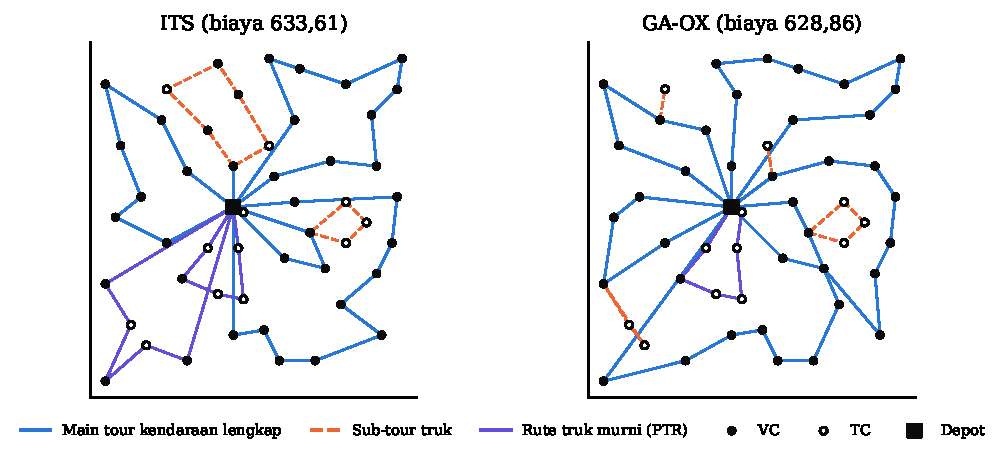
\includegraphics{routes_C01.pdf}
\caption{Solusi terbaik ITS (kiri) dan GA-OX (kanan) pada C01. Garis biru adalah \textit{main tour} kendaraan bertrailer, garis oranye putus-putus adalah \textit{sub-tour} truk setelah trailer diparkir, dan garis ungu adalah rute truk murni.}
\label{fig:routes}
\end{figure*}

Gambar~\ref{fig:routes} memperlihatkan bentuk solusi terbaik ITS dan GA-OX pada C01. Titik hitam adalah VC, lingkaran putih adalah TC, dan kotak di tengah adalah depot. Setiap TC dilayani oleh garis oranye atau ungu, yaitu oleh truk tanpa trailer, sesuai aturan persoalan. ITS memakai \textit{sub-tour} yang lebih panjang dan memuat VC, sedangkan GA-OX memakai \textit{sub-tour} pendek yang hanya berisi TC, sesuai batasan \textit{decoder}. Meski strukturnya berbeda, total jarak keduanya hanya berselisih 4,75 km, atau sekitar 0,75\% (633,61 dan 628,86).

\subsection{Konvergensi}

\begin{figure*}[t]
\centering
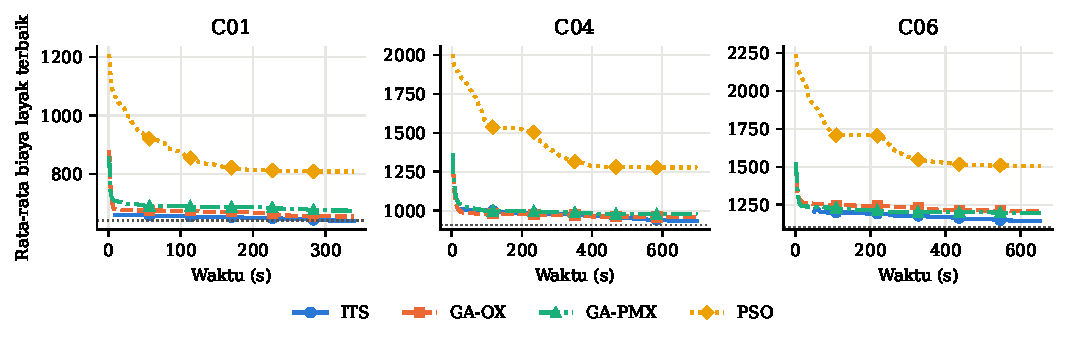
\includegraphics{convergence.pdf}
\caption{Kurva konvergensi: rata-rata (10 run) biaya solusi layak terbaik yang sudah ditemukan, terhadap waktu. Garis titik-titik horizontal adalah nilai acuan. Makin cepat kurva turun dan makin rendah posisi akhirnya, makin baik algoritmanya.}
\label{fig:conv}
\end{figure*}

Gambar~\ref{fig:conv} menunjukkan bagaimana setiap algoritma memperbaiki solusinya seiring waktu pada tiga instance Chao. Sumbu datar adalah waktu sejak run dimulai, dan sumbu tegak adalah biaya rute terbaik yang sudah ditemukan, dirata-ratakan atas 10 run. Kurva hanya bisa turun atau mendatar, karena yang dicatat adalah solusi terbaik sejauh ini.

Ketiga algoritma menunjukkan pola yang berbeda. Kurva GA turun sangat tajam pada beberapa detik pertama, lalu hampir mendatar. Artinya GA cepat menemukan solusi yang cukup baik, tetapi setelah itu sulit memperbaikinya lagi, karena populasi menjadi mirip satu sama lain (konvergensi dini). ITS mulai dari solusi CW yang sudah baik, sehingga garisnya langsung berada di bawah, lalu terus turun perlahan sampai akhir run, terutama pada C04 dan C06. PSO turun paling lambat dan mendatar jauh di atas algoritma lain.

\subsection{Uji statistik}

\begin{table}[t]
\caption{Nilai $p$ uji Wilcoxon \textit{rank-sum} dua sisi pada biaya akhir (10 run per algoritma). Kolom 1: ITS dibanding varian GA/PSO dengan rata-rata terbaik (dalam kurung). Kolom 2: GA-OX dibanding GA-PMX. Kolom 3: varian GA terbaik dibanding PSO. Cetak tebal: $p<0{,}05$.}
\label{tab:stats}
\centering\scriptsize
\begin{tabular}{lccc}
\toprule
Instance & ITS vs terbaik & OX vs PMX & GA vs PSO\\
\midrule
P1 & 1,000 (GA-OX) & 1,000 & 1,000 (GA-OX) \\
P2 & \textbf{0,008} (GA-OX) & 1,000 & 1,000 (GA-OX) \\
P3 & 1,000 (GA-OX) & 1,000 & 1,000 (GA-OX) \\
P4 & 1,000 (GA-OX) & 1,000 & 0,705 (GA-OX) \\
P5 & 1,000 (GA-OX) & 1,000 & 0,450 (GA-OX) \\
P6 & 0,257 (GA-OX) & 1,000 & 0,705 (GA-OX) \\
P7 & 1,000 (GA-OX) & 1,000 & 0,705 (GA-OX) \\
P8 & \textbf{$<$0,001} (GA-OX) & 1,000 & 0,705 (GA-OX) \\
C01 & 0,496 (GA-OX) & 0,070 & \textbf{$<$0,001} (GA-OX) \\
C02 & \textbf{0,007} (GA-OX) & 0,364 & \textbf{$<$0,001} (GA-OX) \\
C03 & 0,597 (GA-OX) & 0,226 & \textbf{$<$0,001} (GA-OX) \\
C04 & 0,070 (GA-OX) & 0,496 & \textbf{$<$0,001} (GA-OX) \\
C05 & \textbf{0,003} (GA-PMX) & 0,762 & \textbf{$<$0,001} (GA-PMX) \\
C06 & \textbf{$<$0,001} (GA-PMX) & 0,496 & \textbf{$<$0,001} (GA-PMX) \\

\bottomrule
\end{tabular}
\end{table}

Tabel~\ref{tab:stats} menguji apakah selisih rata-rata di atas cukup besar untuk tidak dianggap kebetulan. Nilai $p$ di bawah 0,05 berarti kedua algoritma berbeda secara signifikan. Ada tiga temuan:
\begin{itemize}
\item ITS lebih baik secara signifikan daripada GA terbaik pada C02, C05, dan C06. Pada C01, C03, dan C04, selisihnya tidak signifikan ($p=0{,}50$; $0{,}60$; dan $0{,}07$). Pada P2 dan P8, GA justru lebih baik secara signifikan karena selalu menemukan optimum.
\item OX dan PMX tidak berbeda signifikan di instance mana pun ($p\ge 0{,}07$). OX memiliki rata-rata lebih rendah pada C01--C04, dan PMX pada C05--C06.
\item GA lebih baik secara signifikan daripada PSO pada keenam instance Chao. Nilai $p=0{,}00016$ adalah nilai terkecil yang mungkin untuk dua sampel berukuran 10, yaitu ketika semua run GA lebih baik daripada semua run PSO.
\end{itemize}

\subsection{Sensitivitas parameter}\label{sec:sens}

\begin{figure}[t]
\centering
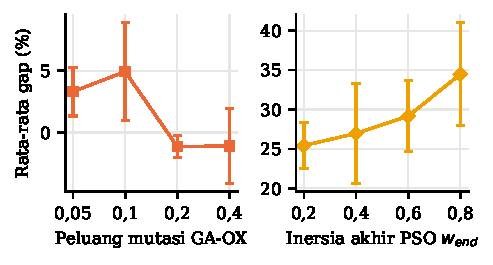
\includegraphics{sensitivity.pdf}
\caption{Pengaruh parameter terhadap rata-rata gap pada C01 (5 run per nilai, garis tegak menunjukkan simpangan baku). Kiri: peluang mutasi GA-OX. Kanan: inersia akhir PSO.}
\label{fig:sens}
\end{figure}

\begin{table}[t]
\caption{Analisis sensitivitas pada C01 (5 run per nilai, batas waktu sama dengan eksperimen utama)}
\label{tab:sens}
\centering\scriptsize
\begin{tabular}{llrrrr}
\toprule
Algoritma & Parameter & Rata-rata & Std & Terbaik & Gap rata-rata (\%)\\
\midrule
GA-OX & peluang mutasi = 0,05 & 661,94 & 12,69 & 642,61 & 3,32 \\
GA-OX & peluang mutasi = 0,1 & 672,25 & 25,32 & 640,73 & 4,93 \\
GA-OX & peluang mutasi = 0,2 & 633,34 & 5,75 & 627,63 & -1,14 \\
GA-OX & peluang mutasi = 0,4 & 633,78 & 19,59 & 605,58 & -1,07 \\
PSO & $w_{\text{end}}$ = 0,2 & 803,56 & 18,73 & 776,04 & 25,43 \\
PSO & $w_{\text{end}}$ = 0,4 & 813,38 & 40,81 & 776,53 & 26,96 \\
PSO & $w_{\text{end}}$ = 0,6 & 827,44 & 28,71 & 788,00 & 29,15 \\
PSO & $w_{\text{end}}$ = 0,8 & 861,67 & 41,76 & 796,95 & 34,50 \\

\bottomrule
\end{tabular}
\end{table}

Gambar~\ref{fig:sens} dan Tabel~\ref{tab:sens} menunjukkan apa yang terjadi bila satu parameter diubah dan parameter lain tetap. Sumbu datar adalah nilai parameter, dan sumbu tegak adalah rata-rata gap. Titik yang lebih rendah berarti hasil lebih baik.

Peluang mutasi berpengaruh besar pada GA. Dengan mutasi 0,05 dan 0,1, rata-rata gap 3,3\% dan 4,9\%. Dengan mutasi 0,2 dan 0,4, rata-rata gap turun menjadi $-1{,}1\%$, yaitu rata-ratanya lebih pendek daripada nilai terbaik di makalah. Mutasi yang terlalu jarang membuat populasi cepat seragam dan pencarian berhenti, sejalan dengan pola konvergensi dini di Gambar~\ref{fig:conv}. Nilai 0,2 yang kami pakai memberi rata-rata yang sama baiknya dengan 0,4 dan simpangan baku terkecil (5,8). Nilai 0,4 menghasilkan solusi terbaik tunggal 605,58, sekitar 5,5\% lebih pendek daripada nilai makalah, tetapi dengan variasi yang jauh lebih besar (simpangan baku 19,6).

Pada PSO, inersia akhir yang lebih kecil memberi hasil lebih baik. Rata-rata gap naik dari 25,4\% ($w_{\text{end}}=0{,}2$) menjadi 34,5\% ($w_{\text{end}}=0{,}8$). Inersia kecil di akhir run membuat partikel lebih fokus di sekitar solusi terbaik. Namun, selisih antarnilai lebih kecil daripada simpangan bakunya, dan gap terbaiknya tetap di atas 25\%. Jadi pemilihan $w_{\text{end}}$ tidak mengubah kesimpulan bahwa PSO tertinggal dari GA.

Run GA-OX dengan mutasi 0,2 di sini memakai pengaturan dan \textit{seed} yang sama dengan eksperimen utama. Biaya akhirnya identik pada empat dari lima \textit{seed}, dan rata-rata \textit{seed} 1--5 adalah 633,3 di sini dan 633,6 di eksperimen utama. Rata-rata 10 \textit{seed} pada Tabel~\ref{tab:summary} (655,3) lebih tinggi karena \textit{seed} 6--10 memberi hasil yang lebih buruk.

\section{Diskusi}\label{sec:diskusi}

\textbf{Mengapa ITS unggul pada instance besar.} ITS bekerja langsung pada struktur rute. Gerakannya dapat memindahkan VC ke dalam \textit{sub-tour}, membuat beberapa \textit{sub-tour} dari satu tempat parkir, dan memilih tempat parkir trailer. Di setiap langkah, ITS memeriksa semua gerakan di sekitar solusi dan mengambil yang terbaik. GA dan PSO tidak memiliki pengetahuan tentang struktur ini. Keduanya hanya mengubah urutan pelanggan, lalu menyerahkan pembentukan rute kepada \textit{decoder} yang lebih sederhana dari model asli. Makin banyak pelanggan, makin besar pengaruh perbedaan ini.

\textbf{Mengapa GA tetap kompetitif.} Untuk satu urutan pelanggan, \textit{decoder} memotongnya menjadi rute secara optimal. Dengan sekitar 0,1 ms per evaluasi, GA mencoba 1,7--4,0 juta urutan per run. Kombinasi ini cukup untuk menyelesaikan semua instance kecil dan sesekali melampaui ITS pada C01 dan C03. Kelemahannya adalah konvergensi dini: setelah beberapa detik populasi seragam dan perbaikan berhenti, sehingga hasil antar-run sangat bervariasi.

\textbf{Mengapa PSO tertinggal.} Representasi \textit{random key} memetakan banyak posisi kontinu ke permutasi yang sama. Perubahan kecil pada posisi sering tidak mengubah permutasi sama sekali, sedangkan perubahan yang melewati batas urutan dapat menukar beberapa pelanggan sekaligus. Arah ``menuju solusi terbaik'' pada persamaan \eqref{eq:vel} karenanya tidak sesuai dengan arah yang bermakna dalam ruang rute. GA dengan OX, sebaliknya, mewariskan potongan urutan kunjungan secara langsung.

\textbf{OX dibanding PMX.} Secara teori OX lebih cocok karena menjaga urutan relatif pelanggan, dan urutan itulah yang menentukan potongan rute di \textit{decoder}. Data kami hanya mendukung hal ini secara lemah: rata-rata OX lebih rendah pada empat dari enam instance Chao, tetapi tidak ada selisih yang signifikan.

\textbf{Keterbatasan.}
\begin{itemize}
\item Anggaran waktu ikut mengukur kecepatan implementasi. ITS berjalan di R, sedangkan GA dan PSO di Python dengan numba, sehingga GA dan PSO mendapat lebih banyak evaluasi per detik. Keunggulan ITS kemungkinan lebih besar bila diimplementasikan dalam bahasa yang sama.
\item \textit{Decoder} hanya mengizinkan satu \textit{sub-tour} per MVR dan tidak menaruh VC di \textit{sub-tour}. Kasus P6 menunjukkan bahwa batasan ini dapat mencegah GA dan PSO mencapai optimum.
\item Hanya 6 dari 21 instance Chao yang diuji, dengan 10 run per algoritma. Uji statistik tidak dikoreksi untuk perbandingan berganda.
\item Parameter GA dan PSO tidak di-\textit{tuning} secara menyeluruh. Analisis sensitivitas hanya dilakukan pada satu instance dengan 5 run.
\item Dengan anggaran waktu, jumlah evaluasi bergantung pada beban komputer saat run berjalan. Pada \textit{seed} yang sama, GA-OX di C01 melakukan sekitar 1,84 juta evaluasi pada eksperimen utama dan 2,17 juta pada analisis sensitivitas, sehingga hasil hanya dapat direproduksi secara statistik, tidak persis per run.
\item Kami memakai aturan armada dan parkir trailer yang sesuai dengan kode dan hasil penulis, bukan teks model MILP secara harfiah (Bagian~\ref{sec:armada}). Batas waktu kerja pengemudi tidak dimodelkan.
\end{itemize}

\section{Kesimpulan}

Heuristik dua fase Davila-Pena dkk.\ \cite{davila2023} dapat direproduksi dengan kode aslinya setelah lima masalah teknis diperbaiki. Biaya CW sama dengan makalah, dan solusi ITS terbaik berada dalam rentang $-1{,}1\%$ sampai $+0{,}4\%$ dari nilai makalah. Dengan waktu yang sama, ITS memberikan rata-rata terbaik pada keenam instance Chao, GA berada di urutan kedua, dan PSO dengan \textit{random key} tertinggal 21--41\%. Pada data nyata yang kecil, GA paling konsisten dan selalu menemukan optimum kecuali pada P6. Variasi \textit{crossover} OX dan PMX tidak menghasilkan perbedaan yang signifikan.

Selama reproduksi, kami juga menemukan dua ketidaksesuaian antara teks model dan hasil makalah, yaitu aturan armada dan parkir trailer di depot. Keduanya mengubah nilai optimum dan perlu ditetapkan secara eksplisit sebelum metode lain dibandingkan dengan makalah ini. Penelitian lanjutan dapat (1) memperluas \textit{decoder} agar mendukung beberapa \textit{sub-tour} dan VC di dalam \textit{sub-tour}, (2) menambahkan \textit{local search} pada GA (algoritma memetika) untuk mengurangi konvergensi dini, dan (3) membandingkan algoritma dengan jumlah evaluasi atau dalam bahasa pemrograman yang sama.

\section*{Pernyataan Kontribusi}

\textcolor{red}{[Diisi oleh kelompok: pembagian kerja tiap anggota, misalnya reproduksi kode R, implementasi GA, implementasi PSO, eksperimen, analisis, dan penulisan laporan.]}

\section*{Pernyataan Penggunaan Alat Bantu AI}

Kami memakai Claude Code (Anthropic) sebagai asisten penulisan kode dan teks. Rinciannya sebagai berikut.
\begin{itemize}
\item \textbf{Reproduksi kode asli.} Kode heuristik makalah ditulis dalam R dengan bagian C++ (Rcpp), sedangkan pemahaman kami terhadap R terbatas. AI kami pakai untuk membaca dan menjelaskan struktur kode R, menyiapkan lingkungan R di macOS, serta men-\textit{debug} galat yang muncul saat kode dijalankan. Galat tersebut adalah pemuatan pustaka khusus Windows, perubahan perilaku operator logika sejak R 4.3, pembacaan memori di luar batas pada fungsi penalti C++, dan dua kesalahan pada skrip reproduksi (Bagian~\ref{sec:metode}). Setiap perbaikan diberi tanda \texttt{[fix]} di kode dan diverifikasi dengan menjalankan ulang instance P1 hingga hasilnya sama dengan makalah (189 km).
\item \textbf{Implementasi GA, PSO, dan perangkat eksperimen.} AI membantu menulis \textit{decoder}, pemeriksa kelayakan, GA, PSO, skrip eksperimen, dan skrip analisis, beserta pengujian otomatisnya.
\item \textbf{Penulisan laporan.} AI membantu menyusun draf teks, tabel, dan gambar dari hasil eksperimen, serta memeriksa detail bibliografi.
\end{itemize}
Seluruh angka dalam laporan berasal dari berkas hasil eksperimen yang dapat diperiksa ulang di repositori. Kami telah meninjau kode, hasil, dan teks, dan kami bertanggung jawab atas kebenarannya.

\begin{thebibliography}{00}
\bibitem{davila2023} L. Davila-Pena, D. R. Penas, and B. Casas-M\'endez, ``A new two-phase heuristic for a problem of food distribution with compartmentalized trucks and trailers,'' \textit{Int. Trans. Oper. Res.}, vol. 30, no. 2, pp. 1031--1064, 2023, doi: 10.1111/itor.13071.
\bibitem{chao2002} I.-M. Chao, ``A tabu search method for the truck and trailer routing problem,'' \textit{Comput. Oper. Res.}, vol. 29, no. 1, pp. 33--51, 2002.
\bibitem{ostermeier2021} M. Ostermeier, T. Henke, A. H\"ubner, and G. W\"ascher, ``Multi-compartment vehicle routing problems: State-of-the-art, modeling framework and future directions,'' \textit{Eur. J. Oper. Res.}, vol. 292, no. 3, pp. 799--817, 2021.
\bibitem{scheuerer2006} S. Scheuerer, ``A tabu search heuristic for the truck and trailer routing problem,'' \textit{Comput. Oper. Res.}, vol. 33, no. 4, pp. 894--909, 2006.
\bibitem{lin2009} S.-W. Lin, V. F. Yu, and S.-Y. Chou, ``Solving the truck and trailer routing problem based on a simulated annealing heuristic,'' \textit{Comput. Oper. Res.}, vol. 36, no. 5, pp. 1683--1692, 2009.
\bibitem{caramia2010a} M. Caramia and F. Guerriero, ``A heuristic approach for the truck and trailer routing problem,'' \textit{J. Oper. Res. Soc.}, vol. 61, no. 7, pp. 1168--1180, 2010.
\bibitem{caramia2010b} M. Caramia and F. Guerriero, ``A milk collection problem with incompatibility constraints,'' \textit{Interfaces}, vol. 40, no. 2, pp. 130--143, 2010.
\bibitem{derigs2013} U. Derigs, M. Pullmann, and U. Vogel, ``Truck and trailer routing problems, heuristics and computational experience,'' \textit{Comput. Oper. Res.}, vol. 40, no. 2, pp. 536--546, 2013.
\bibitem{elfallahi2008} A. El Fallahi, C. Prins, and R. Wolfler Calvo, ``A memetic algorithm and a tabu search for the multi-compartment vehicle routing problem,'' \textit{Comput. Oper. Res.}, vol. 35, no. 5, pp. 1725--1741, 2008.
\bibitem{silvestrin2017} P. V. Silvestrin and M. Ritt, ``An iterated tabu search for the multi-compartment vehicle routing problem,'' \textit{Comput. Oper. Res.}, vol. 81, pp. 192--202, 2017.
\bibitem{prins2004} C. Prins, ``A simple and effective evolutionary algorithm for the vehicle routing problem,'' \textit{Comput. Oper. Res.}, vol. 31, no. 12, pp. 1985--2002, 2004.
\bibitem{davis1985} L. Davis, ``Applying adaptive algorithms to epistatic domains,'' in \textit{Proc. 9th Int. Joint Conf. Artificial Intelligence (IJCAI-85)}, 1985, pp. 162--164.
\bibitem{goldberg1985} D. E. Goldberg and R. Lingle, ``Alleles, loci, and the traveling salesman problem,'' in \textit{Proc. Int. Conf. Genetic Algorithms and Their Applications}, Pittsburgh, PA, 1985, pp. 154--159.
\bibitem{kennedy1995} J. Kennedy and R. Eberhart, ``Particle swarm optimization,'' in \textit{Proc. ICNN'95 Int. Conf. Neural Networks}, vol. 4, 1995, pp. 1942--1948.
\bibitem{shi1998} Y. Shi and R. Eberhart, ``A modified particle swarm optimizer,'' in \textit{Proc. IEEE Int. Conf. Evolutionary Computation}, 1998, pp. 69--73.
\bibitem{bean1994} J. C. Bean, ``Genetic algorithms and random keys for sequencing and optimization,'' \textit{ORSA J. Comput.}, vol. 6, no. 2, pp. 154--160, 1994.
\bibitem{wilcoxon1945} F. Wilcoxon, ``Individual comparisons by ranking methods,'' \textit{Biometrics Bull.}, vol. 1, no. 6, pp. 80--83, 1945.
\end{thebibliography}

\end{document}
